% LAB 3: Functions
%
% CSE/IT 107: Introduction to Programming
% New Mexico Tech
%
% Prepared by Russell White and Christopher Koch
% Spring 2015

% - Functions
%   - Positional and Optional Arguments
%   - Recursion
% - Modules
%   - import statements
%   - main() boilerplate
% - Comments and PEP-8 style
% - Keywords: def
\documentclass[11pt]{cselabheader}
\fancyhead[R]{Lab 3: Functions}
\title{Lab 3: Functions}
\usepgflibrary{fpu}
\newcommand{\pas}{\mathop{\mathrm{pascal}}}

\begin{document}
\pagenumbering{roman}
\maketitle

\begin{figure}[H]
  \centering
  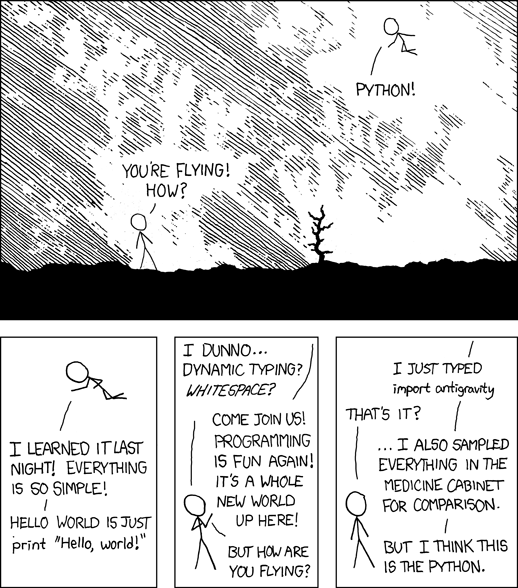
\includegraphics[width=0.85\textwidth]{img/xkcd_python.png}
  \caption{xkcd 353: Python (Source: \url{http://xkcd.com/353})}
\end{figure}

\pagebreak
\hrule
\begin{quotation}
``If you don't think carefully, you might believe that programming is just
typing statements in a programming language.''
\end{quotation}
\begin{flushright}
  --- W. Cunningham
\end{flushright}

\begin{quotation}
``Only ugly languages become popular. Python is the exception.''
\end{quotation}
\begin{flushright}
  --- Donald Knuth
\end{flushright}

\begin{quotation}
``The time you enjoy wasting is not wasted time.''
\end{quotation}
\begin{flushright}
  --- Bertrand Russell
\end{flushright}
\hrule

\tableofcontents

\pagebreak
\pagenumbering{arabic}

\section{Introduction}
\label{sec:intro}

In the previous lab, we showed you simple control flow and how to repeat a piece
of code using \pythoninline{while}. In this lab, we will be learning how to
break a lot of code into smaller, reusable pieces called \emph{functions}.

\section{Making Calculations Shorter}
\label{sec:calc}

We showed you simple Python operators such as \pythoninline{+},
\pythoninline{-}, \pythoninline{*}, \pythoninline{%},
etc in lab 1. There is a small extension to these that you can use to update a
variable:

\begin{pyconcode}
>>> x = 5
>>> x += 3 # same as x = x + 3
>>> x
8
\end{pyconcode}

The available assignment operators are:
\begin{multicols}{2}
\begin{itemize}
  \item \pythoninline{+=} -- addition
  \item \pythoninline{-=} -- subtraction
  \item \pythoninline{*=} -- multiplication
  \item \pythoninline{/=} -- division
  \item \pythoninline{//=} -- integer division
  \item \pythoninline{%=} -- remainder
  \item \pythoninline{**=} -- exponentiation
\end{itemize}
\end{multicols}
They each correspond to the non-assignment version.

\pagebreak
\section{\protect\pythoninline{def}: Functions}
\label{sec:funcs}

So far, we have used functions such as \pythoninline{print()} and
\pythoninline{math.sqrt()}, but we have not yet written our own functions.

Before we dive into that, let's talk about why to write functions. Some reasons:
\begin{itemize}
  \item Instead of writing the same code again, we can just call a function
    containing the code again. (Functions are \emph{reusable}.)
  \item Functions allow us to break our programs into many smaller pieces. This
    also allows us to easily think about each small piece in detail.
  \item Functions allow us to test small parts of our programs while not
    affecting other parts of the program -- this reduces errors in our code.
\end{itemize}

A Python function is simply a ``container'' for a sequence of Python statements
that do some task. Usually, a function does one task and one task only, but it
does it really well. Here's the general form of how to write a function:

\begin{python3code}
def function_name(arg0, arg1, ...):
    # block of code
\end{python3code}

A function can have \emph{zero or more} arguments. For example:

\begin{pyconcode}
>>> def pirate_noises():
...     i = 1
...     while i <= 4:
...         print("Arr!")
...         i += 1
...
\end{pyconcode}

To call this function:

\begin{pyconcode}
>>> pirate_noises()
Arr!
Arr!
Arr!
Arr!
\end{pyconcode}

To call a function, use its name followed by parentheses which contain
comma-separated parameters:

\begin{python3code}
function_name(param0, param1, ...)
\end{python3code}

\begin{itemize}
  \item You must use parentheses both in the function definition and the function
    call, even if there are zero arguments.
  \item The parameter values are substituted for the corresponding arguments to
    the function. I.e. the value of parameter param0 is substituted for argument
    arg0, param1 is substituted for arg1, and so forth.
\end{itemize}

For example:

\begin{pyconcode}
>>> def grocer(num_fruits, fruit_kind):
...     print('Stock: {} cases of {}'.format(num_fruits, fruit_kind))
...
>>> grocer(37, 'kale')
Stock: 37 cases of kale
>>> grocer(0, 'bananas')
Stock: 0 cases of bananas
\end{pyconcode}

\subsection{\protect\pythoninline{return}: Giving back values from a function}

When we used functions from the math module, we were always able to assign the
result of a function to a variable or to print it. For example:

\begin{pyconcode}
>>> import math
>>> x = math.sqrt(16)
>>> print(x)
4.0
\end{pyconcode}

So how do we get a function to give back a value (\emph{return} a value)? We use
the return statement:

\begin{pyconcode}
>>> def square(x):
...     return x**2
...
>>> y = square(5)
>>> print(y)
25
>>> square(4.3)
18.49
\end{pyconcode}

As soon as a \pythoninline{return} statement is reached, the function stops
executing and just returns the value given to it. Any subsequent statements that
are part of the function will be omitted. For example:

\begin{pyconcode}
>>> def wage(hours, base_rate):
...     if hours > 40:
...         ot_pay = (hours - 40) * base_rate * 1.5
...         return base_rate * 40 + ot_pay
...     pay = hours * base_rate
...     return pay
...
>>> wage(40, 10)
400
>>> wage(50, 10)
550
\end{pyconcode}

\begin{itemize}
  \item You can omit the expression after the return and just use a statement of
    this form:

    \begin{python3code}
return
    \end{python3code}

    In this case, the special value \pythoninline{None} is returned from the
    function.

  \item If Python executes your function body and never encounters a
    \pythoninline{return} statement, the effect is the same as a
    \pythoninline{return} with no value at the end of the function body: the
    special value \pythoninline{None} is returned.
\end{itemize}

A function may also call other functions. If we keep using the wage example and
add the ability to calculate the pay after taxes:

\begin{python3code}
def wage(hours, base_rate):
    """Calculate and return weekly pay for a given amount of hours and base rate taking
    into consideration overtime pay at 1.5 times the given rate."""
    if hours > 40:
        ot_pay = (hours - 40) * base_rate * 1.5
        return base_rate * 40 + ot_pay
    pay = hours * base_rate
    return pay

def wage_after_tax(hours, base_rate, tax_rate):
    """Calculate and return weekly pay after taxes for a given amount of hours and a 
    base rate with a flat tax rate."""
    pay = wage(hours, base_rate)
    return pay * (1 - tax_rate)
\end{python3code}

\subsection{Summary}
\label{subsec:funcs.sum}

\begin{itemize}
  \item Function definition syntax:

    \begin{python3code}
def function_name(arg0, arg1, ...):
    # block of code
    \end{python3code}

    Function call syntax:

    \begin{python3code}
function_name(param0, param1, ...)
    \end{python3code}

  \item A function may take zero or more arguments.

  \item A function returns one value. (If the programmer does not specify a
    value, the special value \pythoninline{None} is returned.)

  \item A good resource: \url{https://docs.python.org/3.4/tutorial/controlflow.html#defining-functions}
\end{itemize}


\pagebreak
\section{Conventions}
\label{sec:pep8}

In order to make code more readable, we will start requiring you to comment your
code and follow a style guide. Style guides are often used to make code easy to
read, especially if multiple people are working on a project together. If left
to their own devices, most people start conforming to their own style guide
anyway just by preferring a certain way to write something over another. For
example, common parameter of style guides is the use of a certain number of
spaces for indentation. Also, some people put spaces before each colon, and some
people do not.

\subsection{Style Guide}

We will be using PEP 8 (Python Enhancement Proposal 8 -- Style Guide for Python
Code) found at
\begin{center}
  \url{https://www.python.org/dev/peps/pep-0008/}
\end{center}

Some of the highlights:
\begin{itemize}
  \item 4 space indentation
  \item Function names should be all-lowercase with words separated by underscores.
  \item File/module/package names should have short, all-lowercase names.
  \item Comment your code with useful information. For example,

    \begin{python3code}
x = x + 1 # Increment x
    \end{python3code}

    should be avoided. It is obvious that \pythoninline{x} is being incremented.
    Instead, if you think a comment will improve code comprehension, the
    following can be useful:

    \begin{python3code}
x = x + 1 # Compensate for border
    \end{python3code}

  \item Avoid whitespace where it does not help code legibility. Never put a
    space between a function name and the parentheses when calling a function.

    \begin{python3code}
if x == 4: # do this
    print(x, y)

if x == 4 : # don't do this
    print ( x , y )
    \end{python3code}
\end{itemize}

\pagebreak
\subsection{Commenting Functions}

For commenting on functions, we will be using PEP 257 (Docstring Conventions)
found at
\begin{center}
  \url{https://www.python.org/dev/peps/pep-0257/}
\end{center}

\begin{center}
\bfseries \large You will be required to put a \emph{docstring} at the beginning
of every function that you code from now on.
\end{center}
A docstring is a comment immediately
following the function definition enclosed by triple-double-quotes (\texttt{"""}).

The highlights:
\begin{itemize}
  \item For short functions, do this:

    \begin{python3code}
def midpoint(a, b):
    """Find and return the midpoint of the given a and b."""
    return (a+b)/2
    \end{python3code}

  \item For larger functions or for a longer explanation, follow this style:

    \begin{python3code}
def calculate_weekly_pay(pay_rate, hours, tax_rate):
    """
    Calculate the net pay after taxes given the number of hours worked 
    in a week, a pay rate, and a flat tax rate.
    Takes into consideration overtime pay at 1.5 the pay rate.

    Arguments:
    pay_rate -- rate of pay
    hours -- number of hours worked in one week
    tax_rate -- flat tax rate (for example, 0.15 for 15%)
    """
    pay_before_taxes = hours * pay_rate

    # Add overtime payment if necessary
    if hours > 40:
        pay_before_taxes += (hours - 40) * pay_rate * 0.5

    pay_after_taxes = pay_before_taxes * (1 - tax_rate)
    return pay_after_taxes
    \end{python3code}

\end{itemize}

\pagebreak
\section{Modules}
\label{sec:modules}

A program that is saved in a text file and then run with Python is called a
\emph{script}. As your programs get longer, you may want to split them into
multiple files for easier legibility, maintenance, or abstraction. To do this,
Python supports a way to put definitions (of functions) in a file and use them
in another script or in the interpreter. A file like this is called a
\emph{module}. An example for such a module is the math module we have used
previously. The definitions from a module can be \emph{imported} into other
scripts.

A module is just a file with Python statements in it. A module takes the name of
the file that it is in. For example, imagine we have a file
\texttt{circlemath.py} in our current working directory:

\begin{listing}[H]
\vspace{-0.5em}
\begin{python3code}
import math # importing the math module

def area(radius):
    """Find and return the area of a circle (float) given the radius"""
    return math.pi * radius**2

def circumference(radius):
    """Find and return the circumference of a circle (float) given the radius"""
    return 2 * math.pi * radius
\end{python3code}
\vspace{-1em}
\caption{\texttt{circlemath.py}}
\vspace{-0.5em}
\end{listing}

Then, open the interpreter and import the module:

\begin{pyconcode}
>>> import circlemath
>>> circlemath.circumference(5) # have to use modulename.attributename
31.41592653589793
>>> circlemath.area(5)
78.53981633974483
>>> circlemath.__name__
'circlemath'
\end{pyconcode}

Every module has a \pythoninline{__name__} attribute that contains the name of
the module, except in one special case that we will see soon.

There are other kinds of import statements with different effects:

\begin{pyconcode}
>>> from circlemath import area
>>> area(5) # can just use the attribute imported without modulename.
78.53981633974483
>>> circumference(5) # not defined, because not imported
Traceback (most recent call last):
  File "<input>", line 1, in <module>
NameError: name 'circumference' is not defined
\end{pyconcode}

\begin{pyconcode}
>>> from circlemath import area, circumference # use commas to separate multiple
>>> area(5)
78.53981633974483
>>> circumference(5)
31.41592653589793
\end{pyconcode}

\begin{pyconcode}
>>> from circlemath import * # import all definitions made
>>> area(5)
78.53981633974483
>>> circumference(5)
31.41592653589793
\end{pyconcode}

\begin{pyconcode}
>>> from circlemath import area as carea
>>> carea(5)
78.53981633974483
\end{pyconcode}

The last option is rather frowned upon; we would prefer you to use
\pythoninline{circlemath.area} instead as it is more descriptive.

You may also rename a module upon importing it:

\begin{pyconcode}
>>> import circlemath as cmath
>>> cmath.area(5)
78.53981633974483
\end{pyconcode}


\begin{infobox}{Convention (PEP 8)}
  Always put \pythoninline{import} statements at the beginning of a file in the
  following order:
  \begin{enumerate}
    \item Built-in standard library modules
    \item Third-party modules (e.g. matplotlib)
    \item Self-written modules
  \end{enumerate}
  Put a blank line between each group of imports.
\end{infobox}

\subsection{Using Modules as Scripts and Boilerplate}

If there is code in your module that is not a function definition, Python will
run it just once when the module is imported. For example, take the file
\texttt{mid.py}:

\begin{listing}[H]
  \vspace{-0.5em}
\begin{python3code}
def midpoint(a, b):
    """Find and return the midpoint of two numbers."""
    return (a+b)/2

print('Midpoint of {} and {} is {:.2f}.'.format(5, 10, midpoint(5, 10)))
\end{python3code}
  \vspace{-1em}
  \caption{\texttt{mid.py}}
  \vspace{-0.5em}
\end{listing}

\begin{pyconcode}
>>> import mid
Midpoint of 5 and 10 is 7.50.
\end{pyconcode}

The same will happen if you run the module like a script:

\begin{bashcode}
$ python3 mid.py
Midpoint of 5 and 10 is 7.50.
\end{bashcode}

However, this can be rather annoying to deal with, for example if you wrote a
script with a bunch of functions a while ago and you just want to use the
functions you wrote, but do not want the other code to run when you're using
them -- you just want the functions. You can achieve this!

When you run a module as a script, the modules \pythoninline{__name__} attribute
is not set to the module's name, but to \pythoninline{"__main__"}. Hence, the
following code in \texttt{mid.py} will do the following:

\begin{listing}[H]
  \vspace{-0.5em}
\begin{python3code}
def midpoint(a, b):
    """Find and return the midpoint of two numbers."""
    return (a+b)/2

print(__name__) # just for demonstration, do not put this in real programs

if __name__ == "__main__":
    print('Midpoint of {} and {} is {:.2f}.'.format(5, 10, midpoint(5, 10)))
\end{python3code}
  \vspace{-1em}
  \caption{\texttt{mid.py}}
  \vspace{-0.5em}
\end{listing}

\begin{pyconcode}
>>> import mid
mid
\end{pyconcode}

\begin{bashcode}
$ python3 mid.py
__main__
Midpoint of 5 and 10 is 7.50.
\end{bashcode}

However, sometimes you may want to import the module \emph{and} run it as if it
were a script. To enable us to do so, we usually put the script code in a
function called \pythoninline{main()}:

\begin{listing}[H]
  \vspace{-0.5em}
\begin{python3code}
def midpoint(a, b):
    """Find and return the midpoint of two numbers."""
    return (a+b)/2

def main():
    print('Midpoint of {} and {} is {:.2f}.'.format(5, 10, midpoint(5, 10)))

if __name__ == "__main__":
    main()
\end{python3code}
  \vspace{-1em}
  \caption{\texttt{mid.py} -- perfect example}
  \vspace{-0.5em}
\end{listing}

\begin{pyconcode}
>>> import mid
>>> mid.main() # if we want to
Midpoint of 5 and 10 is 7.50.
\end{pyconcode}

\begin{bashcode}
$ python3 mid.py
Midpoint of 5 and 10 is 7.50.
\end{bashcode}

We call this combination of the if-statement and the
\pythoninline{main()} function \emph{boilerplate code}.

\begin{infobox}{Boilerplate Requirement}
  Please put \textbf{any} code that is not part of a function inside the
  boilerplate if-statement so that \emph{every} one of your scripts can also be
  used as a module. This will be required for every lab from now on.

  Wrong:

  \begin{python3code}
print("Hello World!")
  \end{python3code}

  Right:

  \begin{python3code}
def main():
    print("Hello World!")

if __name__ == "__main__":
    main()
  \end{python3code}
\end{infobox}

\subsection{The \protect\pythoninline{dir()} Function}

Use the \pythoninline{dir()} function to get a list of every attribute --
variables, functions, and other things you do not know about yet -- that is part
of a module. For example for the circlemath module we wrote earlier:

\begin{pyconcode}
>>> import circlemath
>>> dir(circlemath)
['__name__', 'area', 'circumference']
>>> import mid
>>> dir(mid)
['__name__', 'midpoint']
>>> import math
>>> dir(math)
['__doc__', '__file__', '__loader__', '__name__', '__package__', '__spec__', 'acos',
'acosh', 'asin', 'asinh', 'atan', 'atan2', 'atanh', 'ceil', 'copysign', 'cos', 'cosh',
'degrees', 'e', 'erf', 'erfc', 'exp', 'expm1', 'fabs', 'factorial', 'floor', 'fmod',
'frexp', 'fsum', 'gamma', 'hypot', 'isfinite', 'isinf', 'isnan', 'ldexp', 'lgamma',
'log', 'log10', 'log1p', 'log2', 'modf', 'pi', 'pow', 'radians', 'sin', 'sinh', 'sqrt',
'tan', 'tanh', 'trunc']
\end{pyconcode}

\pagebreak
\subsection{Summary}
\label{subsec:modules.sum}

\begin{itemize}
  \item Syntax:

    \begin{python3code}
import modname1, modname2 # use: modname1.attributename
import modname3 as othermodname # use: othermodname.attributename
from modname import attribute1, attribute2 # use: attribute1, attribute2
from modname import * # use: attributename
from modname import attribute as otherattribute # use: otherattribute
    \end{python3code}

    Attributes can be functions defined in the module or variables defined in
    the module. A special attribute is \pythoninline{__name__}, which contains
    the name of the module unless the module is executed as a script.

  \item Every script is a module whose name is the filename of the script.

  \item If a module is imported, its \pythoninline{__name__} attribute is a
    variable that contains the module name. If a module is run as a script, its
    \pythoninline{__name__} attribute contains \pythoninline{"__main__"}. With
    this, you can have code that only runs if a module is run like a script.

    We call that boilerplate code:

    \begin{python3code}
def main():
    # stuff that only runs if module is run as a script

if __name__ == "__main__":
    main()
    \end{python3code}

  \item Use \pythoninline{dir()} to get a list of every attribute -- every
    variable and function (and other things that you do not know about yet) --
    that is part of a particular module.

  \item A good resource:

    \begin{center}
      \url{https://docs.python.org/3.4/tutorial/modules.html}
    \end{center}

\end{itemize}


\pagebreak
\section{Recursion}
\label{sec:rec}

Recursion is the idea of a function calling itself. This can be useful in a wide
variety of situations, but it can also be easy to misuse. Let us first look at a
good example:
\begin{python3code}
def factorial(n):
    """Compute and return n! recursively by knowing that n! = n * (n-1)! for n > 1
    and 1! = 1 and 0! = 1"""
    if n <= 1:
        return 1
    else
        return n * factorial(n-1)
\end{python3code}

Notice that this is just another way to repeat a statement, similar to a loop.
In a loop, we have to specify when to stop repeating something, and we have to
do the same thing with recursion; otherwise, it would run forever.

As an example, this is how the function plays out:
\[ f(5) = 5 * f(4) = 5 * 4 * f(3) = 5 * 4 * 3 * f(2) = 5 * 4 * 3 * 2 * f(1) = 5
* 4 * 3 * 2 * 1 = 120 \]

As an example, see this simple \textbf{\emph{bad}} case of recursion:

\begin{python3code}
def test():
    """BAD example of recursion."""
    test()
\end{python3code}

If this function is called, it will continue to call itself infinitely until
Python prints out an error message and quits. This is because the function calls
itself every time it is called -- there is no case where the function ends
without calling itself again. The case in which the recursion ends is called a
\emph{base case} and it is important to include one in every recursive function.
Here is a modified version of the above code that allows the initial call to
specify a value limiting how many times the recursive call should be made:

\begin{python3code}
def test(x):
    if x > 0:
        test(x - 1)
\end{python3code}

\subsection{Summary}
\label{subsec:adv.sum}

\begin{itemize}
  \item A function may call itself. This is called recursion.
  \item Always need a base case, or the function will keep calling itself
    forever.
\end{itemize}

\pagebreak

\section{Exercises}

\begin{warningbox}{New Requirements}
  Please be aware of the new coding requirements laid out by
  Section~\ref{sec:pep8} (PEP 8 and PEP 257) and Section~\ref{sec:modules}
  (boilerplate code).
\end{warningbox}

\begin{warningbox}{Install}
  Please have the \pythoninline{matplotlib} module installed on your computer
  before next lab. If you installed Anaconda Python, you already have it. Please
  come see a TA if you are having problems with the installation!
\end{warningbox}


\begin{ex}[geometry.py, triangle.py, regularpolygons.py, rectangle.py, circle.py]
  Write a Python script that lets the user do some basic
  geometry calculations. Your output should look something like the following.

  The majority of the output must be calculated by your program using a function
  for each kind of calculation. \emph{The output given below is just an example.
  Your program needs to perform the calculations for the numerical values read
  from the keyboard.}

  \begin{verbatimcode}
Welcome to Wile E. Coyote's Geometry Calculator!

Enter height of a rectangle >>> 2
Enter width of a rectangle >>> 3

The area of a rectangle with height 2 and width 3 is 6.
The perimeter of a rectangle with height 2 and width 3 is 10.
The length of the diagonal of a rectangle with height 2 and width 3 is 3.605551.

Enter the radius of a circle >>> 2

The area of a circle with radius 2.00 is 12.57.
The circumference of a circle with radius 2.00 is 12.57.

Enter the height of a right triangle >>> 1
Enter the base of a right triangle >>> 1

The area of a right triangle with height 1.00 and base 1.00 is 0.50.
The perimeter of a triangle with height 1.00 and base 1.00 is 3.41.

Enter the number of sides of a regular polygon as >>> 8
Enter the length of the side of a regular polygon >>> 5

The exterior angle of a regular polygon with 8 sides is 45.00 degrees.
The interior angles of a regular polygon with 8 sides sum to 1080.00 degrees.
Each interior angle of a regular polygon with 8 sides is 135.00 degrees.
The area of a regular polygon with 8 sides each 5.00 long is 120.71.
  \end{verbatimcode}

  \begin{center}
    \bfseries Remember that coding the input part of the program should be your
    \emph{last} step. It is a beginner's mistake to start with that -- you want
    the logic of your functions to be correct before doing any of the input.
    Test your functions with hard-coded values.
  \end{center}

  Please split your program into multiple files. Please create a module each for
  the rectangle functions, the circle functions, the triangle functions, and the
  polygon functions. For each of the modules, use boilerplate code to test the
  functions. Here's an example:

  \begin{python3code}
# Module square (square.py)

def area(side_length):
    """Calculates the area of a square given the length of a side."""
    return side_length ** 2

def perimeter(side_length):
    """Calculates the perimeter of a square given the length of a side."""
    return 4 * side_length

def main():
    side_len = 2
    print('A square with side length {:.2f} has area {:.2f}.'.format(
        side_len, area(side_len)))
    print('A square with side length {:.2f} has perimeter {:.2f}.'.format(
        side_len, perimeter(side_len)))

if __name__ == '__main__':
    main()
  \end{python3code}

  Then, write a script \texttt{geometry.py} that gives the user interface as
  seen in the example above.

  Your program must define the following functions. It is your task to figure
  out the appropriate arguments and return values as well as the code of these
  functions. Notice that the triangle is a \emph{right triangle} where height
  and base are the two legs joined by the 90 degree angle.
  \begin{multicols}{2}
    \begin{itemize}
      \item Module \texttt{triangle}:
        \begin{itemize}
          \item \pythoninline{area}
          \item \pythoninline{hypotenuse}
          \item \pythoninline{perimeter}
        \end{itemize}
      \item Module \texttt{regularpolygons}:
        \begin{itemize}
          \item \pythoninline{exterior_angle}
          \item \pythoninline{interior_angle}
          \item \pythoninline{area}
        \end{itemize}
      \item Module \texttt{rectangle}:
        \begin{itemize}
          \item\pythoninline{area}
          \item \pythoninline{perimeter}
          \item \pythoninline{diagonal}
        \end{itemize}
      \item Module \texttt{circle}:
        \begin{itemize}
          \item \pythoninline{area}
          \item \pythoninline{circumference}
        \end{itemize}
    \end{itemize}
  \end{multicols}

  \emph{Regular Polygons}

  The exterior angle of a regular $n$-polygon is $\frac{360}{n}$, where $n$ is
  the number of sides. The angle is in degrees.

  The sum of the interior angles of a regular $n$-polygon is $180(n-2)$, where the
  angle is in degrees.

  To get one particular interior angle of a regular $n$-polygon, divide by the
  number of angles $n$ to get $\frac{180(n-2)}{n}$.

  Finally, to find the area of a regular $n$-polygon, use the following formula:
  \[ \frac{s^2 \times n}{4 \times \tan\left( \frac{\pi}{n} \right)}, \]
  where $s$ is the length of a side and $n$ is the number of sides.
\end{ex}

\begin{ex}[calls.py] You buy an international calling card to Germany. The
  calling card company has some special offers.

    \begin{enumerate}[(a)]
      \item If you charge your card with less than \$10, you don't get anything
        extra.
      \item For a less than \$25 charge, you get \$3 of extra phone time.
      \item For a less than \$50 charge, you get \$8 of extra phone time.
      \item For a less than \$100 charge, you get \$20 of extra phone time.
      \item For a more than \$100 charge, you get \$25 of extra phone time.
    \end{enumerate}

    Write a function that takes the value the user wants to charge and returns
    the actual value charged.

    In your script, include a way for someone running the script to enter values
    to charge and get the actual value charged.

    Example:

    \begin{verbatimcode}
Enter value you want to charge >>> 24
27 dollars were added to your calling card.
    \end{verbatimcode}
\end{ex}

\begin{ex}[sum.py] Write a recursive function that computes the sum of all the
  numbers from 1 to $n$, where $n$ is the given parameter.
\end{ex}

\begin{ex}[peasants.py] \hfill
  \begin{enumerate}[(a)]
    \item Russian peasant multiplication is a method of multiplying integers in
      which you keep halving one factor while
      doubling the other factor until one of the factors is 1. For example:
      \begin{IEEEeqnarray*}{RCRCL}
        &\quad& 8 &\quad\times\quad& 38 \\
        = && 4 &\quad\times\quad& 76 \\
        = && 2 &\quad\times\quad& 152 \\
        = && 1 &\quad\times\quad& 304
      \end{IEEEeqnarray*}
      Hence, $8 \times 38 = 304$.

      This, of course, becomes a bit more involved if the integer that you keep
      halving is not a power of two. For example, imagine $38$ is the number
      that keeps getting halved:
      \begin{IEEEeqnarray*}{RCRCLCLCL}
        && 8 &\times& 38 \\
        = &\quad& 16 &\times& 19 \\
        = && 32 &\times& 9 &+& 16      &\qquad& \text{$\nicefrac{19}{2} = 9$ with remainder $1$} \\
        = && 64 &\times& 4 &+& 16 + 32 &\qquad& \text{$\nicefrac{9}{2} = 4$ with remainder $1$} \\
        = && 128 &\times& 2 &+& 16 + 32 \\
        = && 256 &\times& 1 &+& 16 + 32 \\
        = && 256 && &+& 16 + 32 \\
        = && 304
      \end{IEEEeqnarray*}

      This is all based on the following recursive definition of multiplication:

      \[ x \times y = \begin{cases}
          \frac{x}{2} \times (2 \times y) & \text{if $x$ is even} \\
          \frac{x-1}{2} \times (2 \times y) + y & \text{if $x$ is odd}
      \end{cases} \]

      Write a \emph{non-recursive} function that implements Russian
      peasant multiplication using a \pythoninline{while} loop. Call this
      function \pythoninline{multiply()}.

    \item The Russian peasant method can also be applied to exponentiation (also
      only for integers):

      \[ x^y = \begin{cases}
          \left( x^2 \right)^{\nicefrac{y}{2}} & \text{if $y$ is even} \\
          x \left( x^2 \right)^{\nicefrac{(y-1)}{2}} & \text{if $y$ is odd} \\
      \end{cases} \]

      This method is also called exponentiation by squaring or the
      square-and-multiply method.

      Write a \emph{recursive} function called \pythoninline{expo()} that
      implements this.

  \end{enumerate}

\end{ex}

\begin{ex}[pascal.py] \hfill

  In Pascal's triangle, each number is the sum of the two numbers directly above
  it. The left and right ends of the triangle always consists of $1$s.

  This recursive rule produces the following triangle:

  \begin{center}
\def\N{9}
\tikz[x=0.75cm,y=0.5cm, 
  pascal node/.style={font=\small}, 
  row node/.style={font=\footnotesize, anchor=west, shift=(180:1)}]
  \path  
    \foreach \n in {0,...,\N} { 
      (-\N/2-1, -\n) node  [row node/.try]{Row \n:}
        \foreach \k in {0,...,\n}{
          (-\n/2+\k,-\n) node [pascal node/.try] {%
            \pgfkeys{/pgf/fpu}%
            \pgfmathparse{round(\n!/(\k!*(\n-\k)!))}%
            \pgfmathfloattoint{\pgfmathresult}%
            \pgfmathresult%
          }}};
  \end{center}

  Write a recursive function \pythoninline{pascal(n, k)} that finds the $k$th
  value of the $n$th row by using the sum of the numbers directly above it.
  We start counting at $0$ for both $n$ and $k$.

  Since we know that the left and right end of the triangle are all $1$s, we
  know that for every row $n$:
  \begin{IEEEeqnarray*}{RCLCL}
    \pas(n, 0) &=& 1 &\qquad& \text{left end} \\
    \pas(n, n) &=& 1 &\qquad& \text{right end}
  \end{IEEEeqnarray*}

  If for example I want to know the $2$nd entry of the $4$th row:

  \begin{IEEEeqnarray*}{RCLCL}
    \pas(4, 2) &=& \pas(3, 1) + \pas(3, 2)  \\
    &=& \pas(2, 0) + \pas(2, 1) + \pas(2, 1) + \pas(2, 2) \\
    &=& 1 + \pas(1, 0) + \pas(1, 1) + \pas(1, 0) + \pas(1, 1) + 1 \\
    &=& 1 + 1 + 1 + 1 + 1 + 1 \\
    &=& 6
  \end{IEEEeqnarray*}
\end{ex}

\section{Submitting}

You should submit your code as a tarball. It should contain all files
used in the exercises for this lab. The submitted file should be named
\begin{center}
  \texttt{cse107\_firstname\_lastname\_lab3.tar.gz}
\end{center}

\begin{center}
  \textbf{Upload your tarball to Canvas before the deadline.}
\end{center}

\listoftheorems

\end{document}
